
\documentclass[12pt]{article}
\pagestyle{empty}
\setlength{\parskip}{0in}
\setlength{\textwidth}{6.8in}
\setlength{\topmargin}{-.5in}
\setlength{\textheight}{9.3in}
\setlength{\parindent}{0in}
\setlength{\oddsidemargin}{-.7cm}
\setlength{\evensidemargin}{-.7cm}

\usepackage{amsmath}
\usepackage{amsthm}
\usepackage{amstext}

\usepackage{graphicx}

\begin{document}


{\bf MAT 105 Quiz 1.1-1.4 (grey) Fall 2009} \hspace{.4in} {\large Name} \hrulefill

\hrulefill

 \emph{Relax.  You have done problems like these before.  Even if these problems look a bit different, just do what you can.  If you're not sure of something, please ask! You may use your calculator.  Please show all of your work and write down as many steps as you can.  Don't spend too much time on any one problem.  Please leave the following grading key blank for me to use.  Do well.  And remember, ask me if you're not sure about something.}

\begin{center}

\begin{tabular}
{|l|c|c|c|c|c|c|c|c|c|c|c|c|} \hline

 Problems & \hspace{5 pt} 1 \hspace{5 pt}  & \hspace{5 pt} 2 \hspace{5 pt} & \hspace{5 pt} 3 \hspace{5 pt} & \hspace{5 pt} 4 \hspace{5 pt} &  \hspace{5 pt} Total  \hspace{5 pt} & &  \hspace{5 pt} Grade \hspace{5 pt}  \\ \hline
&&&&& &&\\  
Points &&&&& &    \hspace{.8in}\% &  \\ 
&&&&& && \\  \hline
Out of & 16 & 16 & 6 & 12 &50 & & \\ \hline

\end {tabular}

\end{center}

\hrulefill

\begin{enumerate}

%%% Old 1.1-1.2, biology (baby), everyday
\item When my nephew was born last year he weighed approximately 8 pounds.  After he was born, he gained 0.5 pounds per week.

\begin{enumerate}
\item Identify and name the variables in the story and state their units.
\vfill
\item Which variable is independent and which is dependent?
\vfill
\item Make a table showing my nephew's weight after 4 weeks, 8 weeks, and 20 weeks.
\vfill
\vfill
\vfill
\item Is the function increasing or decreasing?
\vfill
\end{enumerate}

\newpage

%%% Old 1.2-1.3, wedding, everyday

\item The table shows the cost to hire the Augsburg Jazz Band to play for events.  

\begin{center}
\begin{tabular} {|c|c|c|c|c|} \hline
$M$ & 30 & 60 & 120 & 150 \\ \hline
$C$ & 700 & 800 & 850 & 900 \\ \hline
\end{tabular}
\end{center}

In the table, $M$ = number of minutes played and $C$ = total cost of band  (\$).

\begin{enumerate}
\item What is the cost for hiring a band to play for 60 minutes?

\emph{Don't forget the units.}
\vfill
\item Approximately what is the cost for hiring the band to play for 90 minutes?
\vfill
\item Draw a graph illustrating this information.  \emph{Be sure your axes are labeled and evenly scaled.  Plot the points given and sketch in a smooth line or curve connecting them.}

\vfill
\begin{center}
\scalebox {.8} {
\includegraphics [width = 6in] {graphPaper.pdf}}
\end{center}
\vfill

\item Does your answer to part b agree with your graph?  (Yes or no)  If no, what would a better answer be?
\vfill
\end{enumerate}

\newpage

%%% Old 1.3, Minnesota, fun
\item The 2009 Minnesota State Fair broke many attendance records.  The graph below shows the daily attendance for each day of the fair.

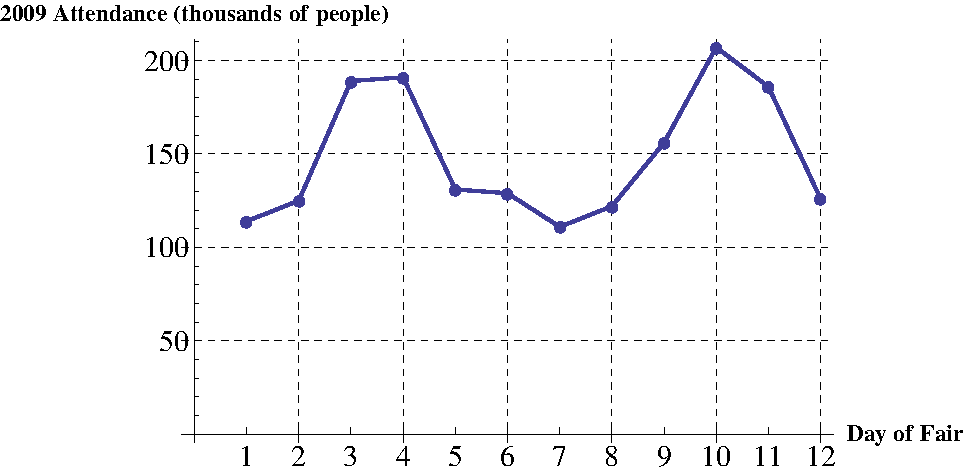
\includegraphics [width = 6in] {stateFair}

\begin{enumerate}
\item What was the approximate attendance for the second day of the fair?
\vfill
\item For how many days was the attendance greater than 150,000 people?
\vfill
\item This year the State Fair started on a Thursday.  What do you think causes the attendance to peak for a given day?  Please write a sentence explaining your answer.
\vfill
\end{enumerate}

\newpage

%%% old 1.4, sports, fun
\item At the 2009 World Swimming Championships, Michael Phelps set a new world record in the 200 meter butterfly.  He swam 200 meters with a time of 1 minute and 51.51 seconds.

\begin{enumerate}
\item Convert his time into (decimal) minutes.
\vfill
\vfill
\item His speed was approximately 107 meters/minute, as you can check.  How fast did he swim in miles per hour?  \emph{Use 1 meter = 3.28 feet and 1 mile = 5,280 feet.}
\vfill
\vfill
\vfill
\end{enumerate}

\end{enumerate}

\end{document}
